# 格子細胞のデコーディング
\subsection{グリッド細胞(Grid Cells)}

\subsubsection{空間基底としてのグリッド細胞}
海馬には場所特異的に発火する\textbf{場所細胞}(place cell)があり,これはO'keefeによって発見された.次にMay-Britt MoserとEdvard Moserが六角形格子状の場所受容野を持つ\textbf{グリッド細胞}(格子細胞, grid cell)を内側嗅内皮質(medial entorhinal cortex; MEC)で発見した.この3人は2014年のノーベル生理学・医学賞を受賞している.
### データについて
格子細胞の活動データはMoser研が公開しており,\url{https://www.ntnu.edu/kavli/research/grid-cell-data}からダウンロードできる.公開されているデータはMATLABのmatファイル形式である.使用するデータ:[10704-07070407_POS.mat](https://github.com/Salad-bowl-of-knowledge/hp/blob/master/_notebooks/data/grid_cells_data/10704-07070407_POS.mat), [10704-07070407_T2C3.mat](https://github.com/Salad-bowl-of-knowledge/hp/blob/master/_notebooks/data/grid_cells_data/10704-07070407_T2C3.mat)

これらのファイルは\url{https://archive.norstore.no/pages/public/datasetDetail.jsf?id=8F6BE356-3277-475C-87B1-C7A977632DA7}からダウンロードできるファイルの一部である.以下では\jl{./data/grid_cells_data/}ディレクトリの下にファイルを置いている.

データの末尾の"POS"と"T2C3"の意味について説明しておく.まず,"POS"はpost, posx, posyを含む構造体でそれぞれ試行の経過時間,x座標, y座標である.座標は$[-50, 50]$で記録されている.1m四方の正方形の部屋で,原点を部屋の中心としている."T2C3"はtがtetrode (テトロード電極) でcがcell (細胞) を意味する.後ろの数字は番号付けである. 
## ラットの行動軌跡と発火の描画
データを読み込む.
\lstinputlisting[language=julia]{./text/appendix/grid-cells-decoding/006.jl}
\lstinputlisting[language=julia]{./text/appendix/grid-cells-decoding/007.jl}
posファイル内の構造は次のようになっている.
\begin{itemize}
\item \jl{pos["post"]}: times at which positions were recorded
\item \jl{pos["posx"]}: x positions
\item \jl{pos["posy"]}: y positions
\item \jl{spk["cellTS"]}: spike times
\end{itemize}
\lstinputlisting[language=julia]{./text/appendix/grid-cells-decoding/009.jl}
行動軌跡を描画する.
\lstinputlisting[language=julia]{./text/appendix/grid-cells-decoding/011.jl}
\begin{figure}[ht]
	\centering
	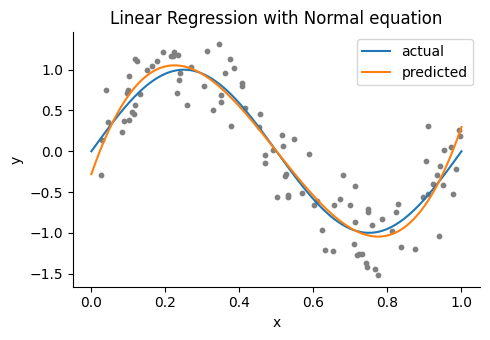
\includegraphics[scale=0.8, max width=\linewidth]{./fig/introduction/linear-regression/cell011.png}
	\caption{cell011.png}
	\label{cell011.png}
\end{figure}
発火を描画するために発火時刻 \jl{spkt} のそれぞれの要素と最も近い \jl{post} のインデックスを求める関数を実装する.
\lstinputlisting[language=julia]{./text/appendix/grid-cells-decoding/013.jl}
\lstinputlisting[language=julia]{./text/appendix/grid-cells-decoding/014.jl}
\lstinputlisting[language=julia]{./text/appendix/grid-cells-decoding/015.jl}
\begin{figure}[ht]
	\centering
	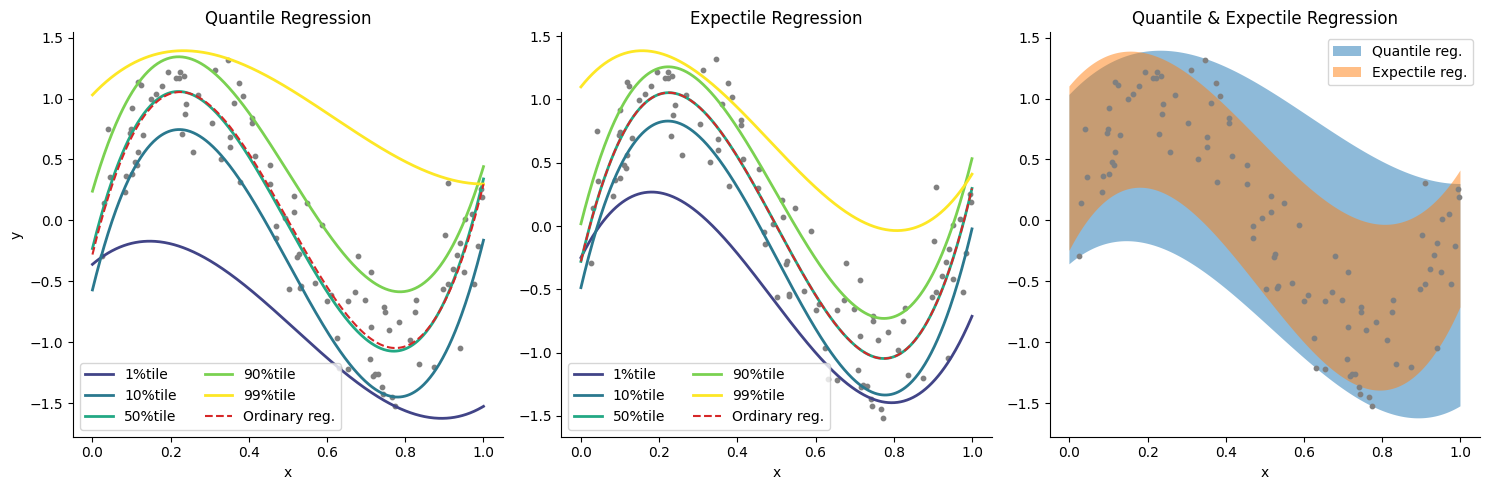
\includegraphics[scale=0.8, max width=\linewidth]{./fig/bayesian-brain/quantile-expectile-regression/cell015.png}
	\caption{cell015.png}
	\label{cell015.png}
\end{figure}
\subsection{発火率マップ}

発火率$\lambda(\boldsymbol{x})$は,場所$\boldsymbol{x}=(x,y)$で記録されたスパイクの回数を,場所$\boldsymbol{x}$における滞在時間(s)で割ることで得られる. 

 
\lambda(\boldsymbol{x})=\frac{\displaystyle \sum_{i=1}^n
g\left(\frac{\boldsymbol{s}_i-\boldsymbol{x}}{h}\right)}{\displaystyle \int_0^T g\left(\frac{\boldsymbol{y}(t)-\boldsymbol{x}}{h}\right)dt} 
 

ただし,$n$はスパイクの回数,$T$は計測時間,$g(\cdot)$はGaussain
Kernel (中身の分子が平均,分母が標準偏差) ,$\boldsymbol{s}_i$は$i$番目のスパイクの発生した位置,$\boldsymbol{y}(t)$は時刻$t$でのラットの位置である.分母は積分になっているが,実際には離散的に記録をするので,累積和に変更し,$dt$を時間のステップ幅(今回は0.02s)とする.

この式の分母はマウスの位置,分子はニューロンが発火したときのマウスの位置についてそれぞれカーネル密度推定 (kernel density estimation)を行うことを意味する.今回はヒストグラムを求め,描画の際にGaussianで平滑化することで計算量を下げることとする.
発火数のヒストグラムを描画する.PyPlotで\jl{hist2D(posx[idx], posy[idx], bins=10, cmap="jet")}などとする方が簡便だが,今回はhistgramの各binの値を用いるために\jl{StatsBase.jl}を用いる.
\lstinputlisting[language=julia]{./text/appendix/grid-cells-decoding/018.jl}
\lstinputlisting[language=julia]{./text/appendix/grid-cells-decoding/019.jl}
\begin{figure}[ht]
	\centering
	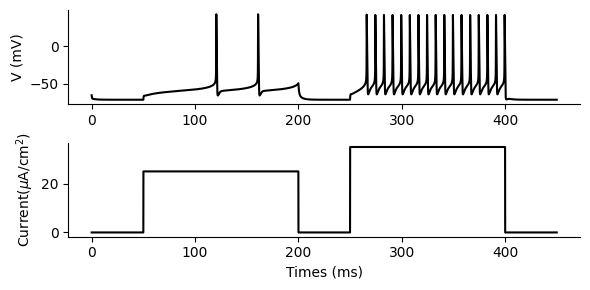
\includegraphics[scale=0.8, max width=\linewidth]{./fig/neuron-model/hodgkin-huxley/cell019.png}
	\caption{cell019.png}
	\label{cell019.png}
\end{figure}
## Autocorrelation Map
2次元の自己相関マップ (autocorrelation map)を描画する.
\lstinputlisting[language=julia]{./text/appendix/grid-cells-decoding/022.jl}
\lstinputlisting[language=julia]{./text/appendix/grid-cells-decoding/023.jl}
\lstinputlisting[language=julia]{./text/appendix/grid-cells-decoding/024.jl}
\begin{figure}[ht]
	\centering
	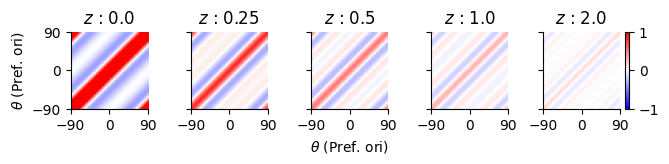
\includegraphics[scale=0.8, max width=\linewidth]{./fig/bayesian-brain/neural-sampling/cell024.png}
	\caption{cell024.png}
	\label{cell024.png}
\end{figure}
\subsection{参考にした文献・サイト}
\begin{itemize}
\item \url{https://github.com/Felix11H/grid_cell_rate_map}
\item \url{https://www.ntnu.edu/kavli/research/grid-cell-data}
\item \url{https://core.ac.uk/download/pdf/30859910.pdf}のSupporting Online Material
\item \url{https://github.com/MattNolanLab/gridcells}
\item \url{https://arxiv.org/pdf/1810.07429.pdf}
\item \url{https://www.diogosantospata.com/gridcells/}
\end{itemize}
